\documentclass{article}
\usepackage{graphicx}
\usepackage{amsmath}
\usepackage{booktabs}
\usepackage{siunitx}
\usepackage{float}
\usepackage{listings}
\usepackage{xcolor}
\usepackage[margin=1in]{geometry}

\lstset{
  language=Matlab,
  basicstyle=\small\ttfamily,
  keywordstyle=\color{blue},
  commentstyle=\color{green!50!black},
  numbers=left,
  numberstyle=\tiny\color{gray},
  frame=single,
  breaklines=true
}

\title{Homework 3 - ET4369 Nyquist Rate Data Converters}
\author{Daniel Tyukov \\ Student Number: 5714699 \\ Electrical Engineering, TU Delft}
\date{March 2026}

\begin{document}

\maketitle
\tableofcontents
\newpage

%% ============================================================
%% PROBLEM 1
%% ============================================================
\section{Spectral Performance Metrics}

\textbf{Given:} ADC output data (\texttt{hw3\_adc\_out.mat}) with $f_s = 100$\,MS/s. The input was a full-scale sinusoidal signal. The ADC has a 10-bit bipolar mid-rise quantizer with full-scale range $[-1, +1]$.

\subsection{Part (a): Spectrum Plot}

The one-sided amplitude spectrum is computed from the 10000-point FFT. Amplitudes are normalized to dBFS using the full-scale amplitude $A_\text{FS} = 1$\,V:
\begin{equation}
    X_\text{dBFS}(k) = 20\log_{10}\!\left(\frac{|X(k)| \cdot 2/N}{A_\text{FS}}\right)
\end{equation}

\begin{figure}[H]
    \centering
    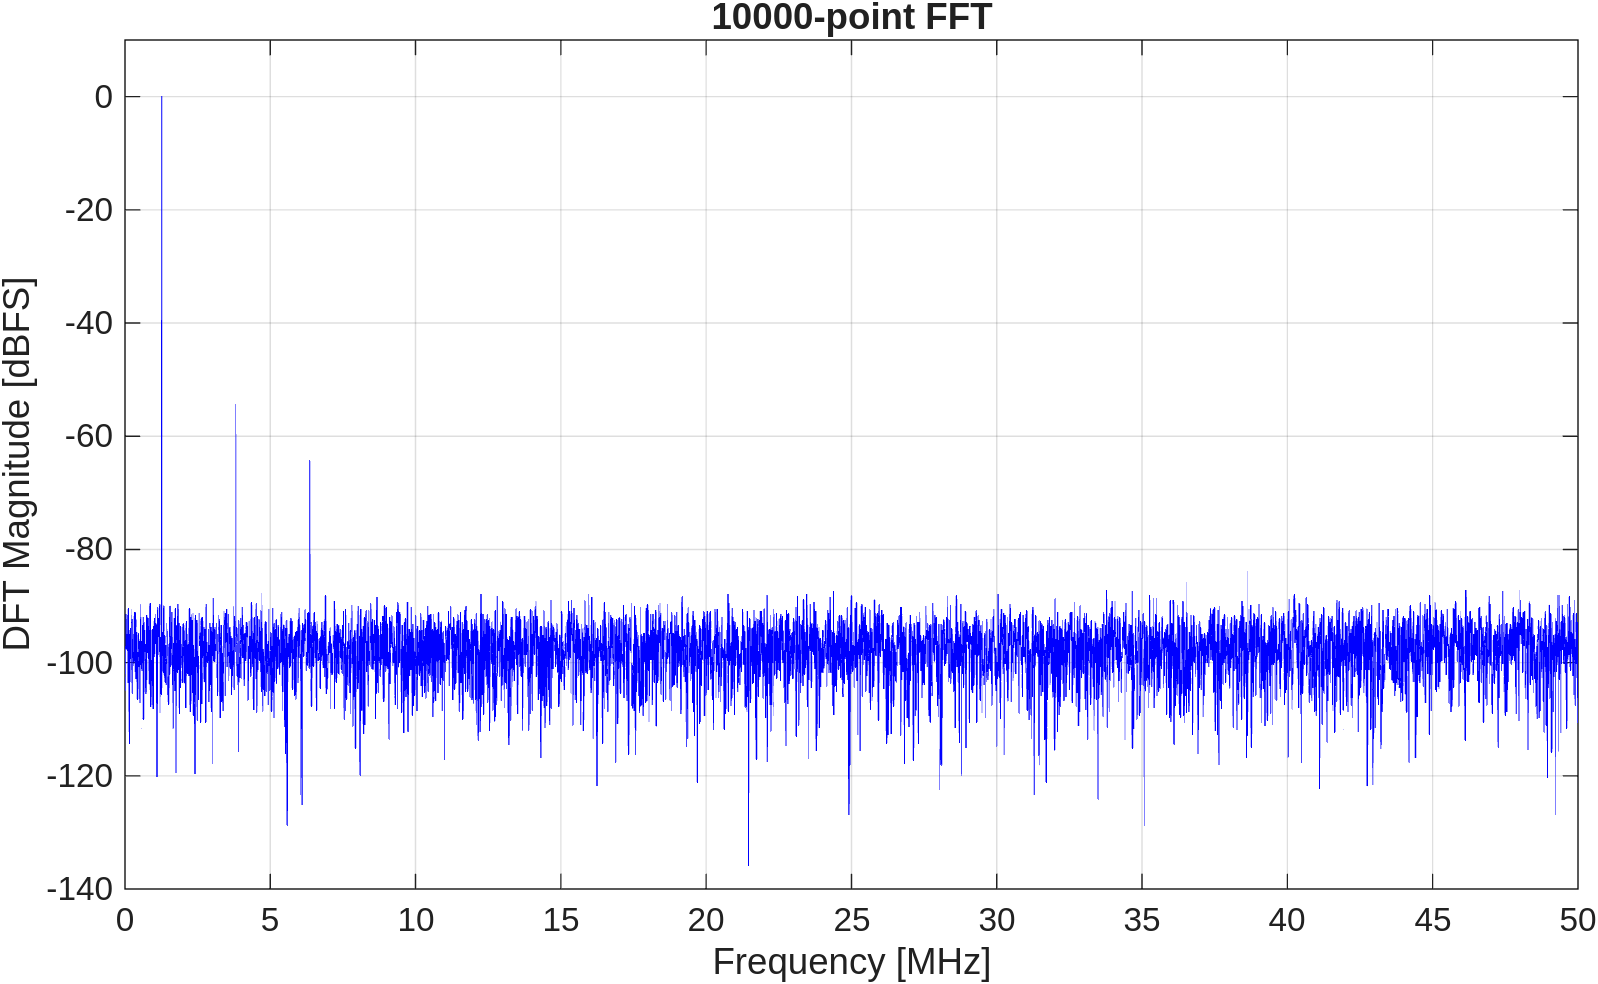
\includegraphics[width=0.9\textwidth]{p1a_spectrum.png}
    \caption{Output spectrum of the 10-bit ADC (10000-point FFT), showing the signal tone at 1.27\,MHz, HD3 at 3.81\,MHz, and HD5 at 6.35\,MHz.}
    \label{fig:p1a}
\end{figure}

\subsection{Part (b): Input Frequency}

The signal frequency is identified from the FFT bin with the largest magnitude (excluding DC):
\begin{equation}
    \boxed{f_\text{in} = 1.27\;\text{MHz} \quad (\text{bin } 127)}
\end{equation}

The signal level is approximately $0$\,dBFS, confirming a full-scale input.

\subsection{Part (c): Performance Metrics}

Metrics are computed using standard IEEE definitions. Harmonics 2 through 7 are identified and their power is separated from noise.

\begin{table}[H]
\centering
\caption{Harmonic levels in the ADC output spectrum.}
\begin{tabular}{@{}cccc@{}}
\toprule
Harmonic & Frequency (MHz) & Level (dBFS) & Notes \\
\midrule
HD2 & 2.54  & $-106.5$ & Even-order \\
HD3 & 3.81  & $-54.5$  & \textbf{Dominant spur} \\
HD4 & 5.08  & $-90.4$  & Even-order \\
HD5 & 6.35  & $-64.3$  & 2nd largest spur \\
HD6 & 7.62  & $-106.5$ & Even-order \\
HD7 & 8.89  & $-103.8$ & --- \\
\bottomrule
\end{tabular}
\label{tab:harmonics}
\end{table}

\begin{table}[H]
\centering
\caption{Summary of spectral performance metrics.}
\begin{tabular}{@{}ll@{}}
\toprule
Metric & Value \\
\midrule
SNR   & 58.94\,dB \\
SNDR  & 52.90\,dB \\
ENOB  & 8.50\,bits \\
THD   & $-54.15$\,dB \\
SFDR  & 54.58\,dB \\
\bottomrule
\end{tabular}
\label{tab:metrics}
\end{table}

The ENOB of 8.50 bits (vs.\ 10-bit quantizer resolution) indicates significant degradation due to distortion and excess noise.

\subsection{Part (d): SFDR-Limiting Non-Ideality}

The SFDR is determined by \textbf{HD3} (3rd harmonic distortion) at $-54.5$\,dBFS. The dominance of odd-order harmonics (HD3 and HD5) is characteristic of a \textbf{symmetric (odd) nonlinearity}, which is typically caused by the signal-dependent on-resistance of the sampling switch:
\begin{equation}
    r_\text{on}(V_\text{in}) = \frac{1}{\mu C_\text{ox} \frac{W}{L} (V_\text{GS} - V_t - V_\text{in})}
\end{equation}

This produces a predominantly cubic transfer function error $\propto V_\text{in}^3$, generating HD3 and HD5.

\subsection{Part (e): Additional Noise Sources}

Comparing measured noise to ideal quantization noise:
\begin{align}
    \text{SQNR}_\text{ideal} &= 6.02 \times 10 + 1.76 = 61.96\;\text{dB} \\
    \text{SNR}_\text{measured} &= 58.94\;\text{dB}
\end{align}

The measured SNR is 3.0\,dB lower than the ideal SQNR. Equivalently, the measured total noise power is approximately $4.1\times$ the ideal quantization noise power:
\begin{equation}
    \frac{P_\text{noise,total}}{P_\text{quant}} = 10^{(61.96 - 58.94)/10} \approx 4.1
\end{equation}

\textbf{Yes, there are additional noise sources} beyond quantization noise. The electronic noise (thermal noise from switches, comparator noise, amplifier noise) contributes approximately $3\times$ the power of the quantization noise alone. The noise floor is elevated by about 3\,dB compared to the ideal $-98.95$\,dBFS floor.

%% ============================================================
%% PROBLEM 2
%% ============================================================
\section{Clock Bootstrapping}

\textbf{Given:} Bootstrapped sampling switch with $C_\text{boot} = C_L = 500$\,fF, $C_\text{par} = 100$\,fF, $V_\text{DD} = 1.8$\,V, $V_t = 0.5$\,V, $WLC_\text{ox} = 50$\,fF, $\mu C_\text{ox} W/L = 10$\,mA/V$^2$. Input range: 0.5\,V to 1\,V.

\subsection{Circuit Operation}

During $\phi_1$ (precharge): $C_\text{boot}$ charges to $V_\text{DD}$, gate of $M_1$ is pulled to ground (off).

During $\phi_2$ (track): $C_\text{boot}$ bottom plate connects to $V_\text{in}$ (source of $M_1$), top plate connects to gate. By charge conservation at the gate node:
\begin{equation}
    C_\text{boot}(V_G - V_\text{in}) + C_\text{par} \cdot V_G = C_\text{boot} \cdot V_\text{DD}
\end{equation}

Solving for $V_\text{GS}$:
\begin{equation}
    V_\text{GS} = V_G - V_\text{in} = \frac{C_\text{boot} \cdot V_\text{DD} - C_\text{par} \cdot V_\text{in}}{C_\text{boot} + C_\text{par}}
    \label{eq:vgs_bootstrap}
\end{equation}

Without $C_\text{par}$, we would have $V_\text{GS} = V_\text{DD}$ (perfectly bootstrapped). The $C_\text{par} \cdot V_\text{in}$ term introduces a residual signal dependence.

\subsection{Part (a): On-Resistance Variation}

Using Eq.~\eqref{eq:vgs_bootstrap} and $r_\text{on} = 1/(\mu C_\text{ox} W/L \cdot V_\text{OV})$ where $V_\text{OV} = V_\text{GS} - V_t$:

\begin{table}[H]
\centering
\begin{tabular}{@{}cccc@{}}
\toprule
$V_\text{in}$ (V) & $V_\text{GS}$ (V) & $V_\text{OV}$ (V) & $r_\text{on}$ ($\Omega$) \\
\midrule
0.5 & 1.417 & 0.917 & 109.1 (minimum) \\
1.0 & 1.333 & 0.833 & 120.0 (maximum) \\
\bottomrule
\end{tabular}
\end{table}

\begin{equation}
    \boxed{\text{Percent increase} = \frac{r_\text{on}(1\,\text{V}) - r_\text{on}(0.5\,\text{V})}{r_\text{on}(0.5\,\text{V})} = \frac{120.0 - 109.1}{109.1} = 10.0\%}
\end{equation}

This can also be derived analytically. Since $r_\text{on} \propto 1/V_\text{OV}$:
\begin{equation}
    \frac{r_\text{on,max}}{r_\text{on,min}} = \frac{V_\text{OV}(0.5\,\text{V})}{V_\text{OV}(1.0\,\text{V})} = \frac{11/12}{5/6} = \frac{11}{10} = 1.10
\end{equation}

\subsection{Part (b): Charge Injection Error Variation}

For fast gating with 50/50 channel charge split, the charge injected onto $C_L$ when $M_1$ turns off:
\begin{equation}
    \Delta V_\text{out} = -\frac{WLC_\text{ox} \cdot V_\text{OV}}{2 \cdot C_L} = -\frac{50\;\text{fF}}{2 \times 500\;\text{fF}} \cdot V_\text{OV} = -\frac{V_\text{OV}}{20}
\end{equation}

Since $V_\text{OV}$ depends on $V_\text{in}$ through Eq.~\eqref{eq:vgs_bootstrap}, the error is signal-dependent:

\begin{table}[H]
\centering
\begin{tabular}{@{}ccc@{}}
\toprule
$V_\text{in}$ (V) & $V_\text{OV}$ (V) & $\Delta V_\text{out}$ (mV) \\
\midrule
0.5 & 0.917 & $-45.83$ \\
1.0 & 0.833 & $-41.67$ \\
\bottomrule
\end{tabular}
\end{table}

\begin{equation}
    \boxed{\Delta V_\text{out,pp} = |{-45.83} - ({-41.67})| = 4.17\;\text{mV}}
\end{equation}

The signal-dependent part of the error arises from $C_\text{par}$: if $C_\text{par} = 0$, then $V_\text{OV}$ would be constant ($V_\text{DD} - V_t$), and the charge injection would be purely a fixed offset (no signal-dependent variation).

%% ============================================================
%% PROBLEM 3
%% ============================================================
\section{Relationship between INL and SFDR}

\textbf{Given:} Output spectrum of an 11-bit A/D converter for a full-scale sinusoidal input (65536-point FFT shown on page~2 of the assignment).

\subsection{Part (a): Maximum INL (Cubic Bow)}

From the spectrum, the dominant spur is HD3 at approximately $-40$\,dBFS, giving $\text{SFDR} \approx 40$\,dB.

For a cubic INL with endpoint correction, $\text{INL}(u) = A_3(u^3 - u)$ where $u \in [-1, 1]$ is the normalized code. The maximum occurs at $u = \pm 1/\sqrt{3}$ with value $|u^3 - u|_\text{max} = 2/(3\sqrt{3})$. The relationship between INL and HD3:
\begin{equation}
    \text{HD3} = \frac{3\sqrt{3} \cdot \text{INL}_\text{max}}{4 \cdot 2^B}
\end{equation}

Rearranging:
\begin{equation}
    \text{INL}_\text{max} = \frac{4 \cdot 2^B}{3\sqrt{3} \cdot 10^{\text{SFDR}/20}} = \frac{4 \times 2048}{5.196 \times 100}
\end{equation}
\begin{equation}
    \boxed{\text{INL}_\text{max} \approx 15.8\;\text{LSB}}
\end{equation}

\subsection{Part (b): Electronic Noise Standard Deviation}

The ideal quantization noise floor for an 11-bit ADC with a 65536-point FFT:
\begin{equation}
    \text{Floor}_\text{ideal} = -\text{SQNR} - 10\log_{10}(N/2) = -67.98 - 45.15 = -113.13\;\text{dBFS}
\end{equation}

From the spectrum, the measured noise floor is approximately $-100$\,dBFS. The total noise power per bin is $10^{13.13/10} \approx 20.6\times$ the ideal quantization noise, meaning the electronic noise power is about $19.6\times$ the quantization noise.

\begin{equation}
    \sigma_\text{electronic} = \Delta \sqrt{\frac{P_\text{elec}}{P_\text{quant}} \cdot \frac{1}{12}} = \Delta \sqrt{\frac{19.6}{12}}
\end{equation}
\begin{equation}
    \boxed{\sigma_\text{electronic} \approx 1.28\;\text{LSB}}
\end{equation}

\subsection{Part (c): Effective Number of Bits}

The SNDR is dominated by distortion (HD3 at $-40$\,dBFS relative to the signal):
\begin{equation}
    \text{SNDR} = 10\log_{10}\!\left(\frac{P_\text{signal}}{P_\text{noise} + P_\text{distortion}}\right) \approx 39.9\;\text{dB}
\end{equation}

Since the distortion power ($10^{-4} \cdot P_\text{signal}$) greatly exceeds the noise power ($\sim 10^{-5.5} \cdot P_\text{signal}$), SNDR $\approx$ SFDR.

\begin{equation}
    \boxed{\text{ENOB} = \frac{\text{SNDR} - 1.76}{6.02} = \frac{39.9 - 1.76}{6.02} \approx 6.3\;\text{bits}}
\end{equation}

\subsection{Part (d): INL and SFDR in a Commercial Product}

\textbf{Paper:} S.-C.~Lee et al., ``A 10-bit 205-MS/s 1.0-mm$^2$ 90-nm CMOS Pipeline ADC for Flat Panel Display Applications,'' \textit{IEEE J. Solid-State Circuits}, vol.~42, no.~12, pp.~2688--2695, Dec.~2007.

\textbf{Key data from the paper:}
\begin{itemize}
    \item Fig.~14(a): Differential input ($1.0$-$V_\text{PP}$): DNL $= \pm 0.5$\,LSB, INL $= \pm 0.5$\,LSB.
    \item Fig.~14(b): Single-ended input ($1.0$-$V_\text{PP}$): INL $= \pm 0.9$\,LSB with a clear \textbf{cubic S-shaped bow}. The distortion from the front-end switched source follower causes the symmetrical bend (noted by the authors on p.~2694).
    \item Fig.~10(b): SFDR vs.\ input frequency at 205\,MS/s for single-ended input shows SFDR $\approx 62$\,dBc around $f_\text{in} = 70$\,MHz.
    \item Fig.~11(d): At $f_\text{in} = 79$\,MHz, SFDR $= 61.8$\,dBc is explicitly labeled.
\end{itemize}

Using the smooth average INL amplitude of $\pm 0.9$\,LSB from Fig.~14(b):
\begin{equation}
    \text{HD3} = \frac{3\sqrt{3} \times 0.9}{4 \times 2^{10}} = \frac{4.677}{4096} = 0.001142
\end{equation}
\begin{equation}
    \text{SFDR}_\text{estimated} = -20\log_{10}(0.001142) \approx 58.8\;\text{dB}
\end{equation}

From Fig.~10(b), the measured SFDR at $\sim$70\,MHz is approximately 62\,dBc.

\begin{equation}
    \boxed{\text{SFDR}_\text{from INL} \approx 58.8\;\text{dBc} \quad\text{vs.}\quad \text{SFDR}_\text{measured} \approx 62\;\text{dBc}}
\end{equation}

The 3.2\,dB difference indicates reasonable agreement. The INL-based estimate is slightly pessimistic, which is expected: the smooth cubic fit overestimates the true harmonic content since the actual INL also contains random (non-cubic) components that don't coherently add to HD3. Nevertheless, the cubic INL model correctly predicts the SFDR to within a few dB, confirming that the cubic nonlinearity from the switched source follower is the dominant distortion mechanism.

%% ============================================================
%% PROBLEM 4
%% ============================================================
\section{Switch Nonidealities}

\textbf{Given:} Switched-capacitor circuit with all NMOS switches: $W = 10\;\mu$m, $L = 0.2\;\mu$m, $C_\text{ox} = 10$\,fF/$\mu$m$^2$, $V_t = 0.4$\,V, $C_\text{ol} = 0.1$\,fF/$\mu$m. $C_1 = 1$\,pF, $C_2 = 2$\,pF. Fast gating assumed; settling dynamics ignored.

\subsection{Device Parameters}

\begin{table}[H]
\centering
\begin{tabular}{@{}ll@{}}
\toprule
Parameter & Value \\
\midrule
$WLC_\text{ox}$ & $10 \times 0.2 \times 10 = 20$\,fF \\
$C_\text{ov}$ (overlap per terminal) & $C_\text{ol} \times W = 0.1 \times 10 = 1$\,fF \\
\bottomrule
\end{tabular}
\end{table}

\subsection{Circuit Operation}

During $\phi_1$: left $\phi_1$ switch connects 1\,V source to $V_1$ (charges $C_1$), right $\phi_1$ switch connects $V_2$ to its reference. The $\phi_2$ switch is off.

At $t = t_1$: $\phi_1$ turns off (both $\phi_1$ switches open simultaneously).

During $\phi_2$: $\phi_2$ switch connects $V_1$ to $V_2$ (charge sharing between $C_1$ and $C_2$).

At $t = t_2$: $\phi_2$ turns off.

\subsection{Part (e): Standard Deviation of $V_1$ at $t_1$ and $t_2$}

\textbf{At $t_1$} ($\phi_1$ opens): $V_1$ was tracking the 1\,V source through the left $\phi_1$ switch. The sampled $kT/C$ noise:
\begin{equation}
    \sigma(V_1)\big|_{t_1} = \sqrt{\frac{kT}{C_1}} = \sqrt{\frac{4.14 \times 10^{-21}}{1 \times 10^{-12}}}
\end{equation}
\begin{equation}
    \boxed{\sigma(V_1)\big|_{t_1} = 64.4\;\mu\text{V}_\text{rms}}
\end{equation}

\textbf{At $t_2$} ($\phi_2$ opens): During $\phi_2$, $V_1$ and $V_2$ were connected through the switch with both $C_1$ and $C_2$ floating. The total charge $Q = C_1 V_1 + C_2 V_2$ is conserved. The noise on $V_1$ decomposes into:

\begin{itemize}
    \item \textbf{Common-mode noise} (from $\phi_1$ sampling): The total charge carries noise $\sigma^2(Q) = kT(C_1 + C_2)$, contributing $\sigma^2(V_\text{cm}) = kT/(C_1 + C_2)$ to $V_1$.
    \item \textbf{Differential noise} (from $\phi_2$ switch): By equipartition, $\sigma^2(\delta V_1) = kT \cdot C_2/[C_1(C_1 + C_2)]$.
\end{itemize}

These are independent, so:
\begin{equation}
    \sigma^2(V_1)\big|_{t_2} = \frac{kT}{C_1 + C_2} + \frac{kT \cdot C_2}{C_1(C_1 + C_2)} = \frac{kT}{C_1}
\end{equation}

\begin{equation}
    \boxed{\sigma(V_1)\big|_{t_2} = \sqrt{\frac{kT}{C_1}} = 64.4\;\mu\text{V}_\text{rms}}
\end{equation}

The result is the \textbf{same} at both times. This is a fundamental property of switched-capacitor circuits: the $kT/C$ noise on a node depends only on the capacitance at that node, regardless of the switching history. The noise ``reset'' during $\phi_2$ (charge sharing with $C_2$) exactly compensates for the additional noise injected by the $\phi_2$ switch.

\subsection{Part (f): Charge Injection on $V_1$ at $t_1$}

When the left $\phi_1$ switch turns off, the channel charge splits 50/50 (fast gating):
\begin{align}
    V_\text{GS} &= 1.8\;\text{V} - 1.0\;\text{V} = 0.8\;\text{V} \\
    V_\text{OV} &= V_\text{GS} - V_t = 0.8 - 0.4 = 0.4\;\text{V} \\
    Q_\text{ch} &= WLC_\text{ox} \cdot V_\text{OV} = 20\;\text{fF} \times 0.4\;\text{V} = 8\;\text{fC}
\end{align}

Half of the channel charge is injected onto $C_1$:
\begin{equation}
    \Delta V_1 = -\frac{Q_\text{ch}}{2 \cdot C_1} = -\frac{8\;\text{fC}}{2 \times 1\;\text{pF}} = -4.0\;\text{mV}
\end{equation}

\begin{equation}
    \boxed{V_1(t_1) = 1.0 - 0.004 = 0.996\;\text{V}}
\end{equation}

\subsection{Part (g): Clock Feedthrough on $V_1$ at $t_1$}

When $\phi_1$ drops from 1.8\,V to 0\,V, the gate voltage change couples to $V_1$ through the overlap capacitance $C_\text{ov}$:
\begin{equation}
    \Delta V_1 = \Delta V_\text{gate} \cdot \frac{C_\text{ov}}{C_\text{ov} + C_1} = (-1.8\;\text{V}) \cdot \frac{1\;\text{fF}}{1\;\text{fF} + 1000\;\text{fF}}
\end{equation}

\begin{equation}
    \Delta V_1 = -1.8 \times \frac{1}{1001} = -1.80\;\text{mV}
\end{equation}

\begin{equation}
    \boxed{V_1(t_1) = 1.0 - 0.00180 = 0.99820\;\text{V}}
\end{equation}

Note that charge injection ($-4.0$\,mV) is the larger effect compared to clock feedthrough ($-1.8$\,mV). In practice, both contribute simultaneously, giving a total error of approximately $-5.8$\,mV.

%% ============================================================
%% PROBLEM 5
%% ============================================================
\section{Boxcar Sampling}

\textbf{Paper:} H.~Gao, R.~M.~Walker, P.~Nuyujukian, K.~A.~A.~Makinwa, K.~V.~Shenoy, B.~Murmann and T.~H.~Meng, ``HermesE: A 96-Channel Full Data Rate Direct Neural Interface in 0.13\,$\mu$m CMOS,'' \textit{IEEE J. Solid-State Circuits}, pp.~1043--1055, Apr.~2012.

\subsection{Part (h): Derivation of Equation (2)}

Starting from Eq.~(1) of the paper, the boxcar integrator output is:
\begin{equation}
    Q_\text{in2,CT}(t) = \int_{t - DT_s}^{t} I_\text{out1d}(t')\, dt'
    \label{eq:boxcar_time}
\end{equation}
where $D$ is the duty cycle of the $\Phi_1$ sampling phase and $T_s = 1/f_s$ is the SC clock period.

This is a convolution of $I_\text{out1d}(t)$ with a rectangular window:
\begin{equation}
    h(\tau) = \begin{cases} 1, & 0 \leq \tau \leq DT_s \\ 0, & \text{otherwise} \end{cases}
\end{equation}

Taking the Fourier transform:
\begin{align}
    H(\omega) &= \int_0^{DT_s} e^{-j\omega\tau}\, d\tau = \frac{1 - e^{-j\omega DT_s}}{j\omega}
\end{align}

Factoring out $e^{-j\omega DT_s/2}$:
\begin{align}
    H(\omega) &= e^{-j\omega DT_s/2} \cdot \frac{e^{j\omega DT_s/2} - e^{-j\omega DT_s/2}}{j\omega} \nonumber \\
    &= e^{-j\omega DT_s/2} \cdot \frac{2\sin(\omega DT_s/2)}{\omega}
\end{align}

Since $Q_\text{in2,CT}(\omega) = I_\text{out1d}(\omega) \cdot H(\omega)$, taking the magnitude:

\begin{equation}
    \boxed{\frac{|Q_\text{in2,CT}(\omega)|}{|I_\text{out1d}(\omega)|} = \frac{2\left|\sin\!\left(\frac{\omega DT_s}{2}\right)\right|}{\omega}}
    \label{eq:eq2_derived}
\end{equation}

This is equation~(2) of the paper. In the baseband ($\omega DT_s/2 \ll 1$), the $\operatorname{sinc}$ response is approximately flat, providing inherent anti-alias filtering by attenuating high-frequency noise components before they fold into the signal band.

\subsection{Part (i): Verification of the 3.4$\times$ ENBW Advantage}

\subsubsection{Boxcar (sinc) prefilter ENBW}

The power transfer function is $|H(f)|^2 = (DT_s)^2 \operatorname{sinc}^2(f \cdot DT_s)$, with DC gain $|H(0)|^2 = (DT_s)^2$. The effective noise bandwidth:
\begin{equation}
    \text{ENBW}_\text{boxcar} = \frac{1}{|H(0)|^2} \int_0^{\infty} |H(f)|^2\, df = \int_0^{\infty} \operatorname{sinc}^2(f \cdot DT_s)\, df = \frac{1}{2\, DT_s}
    \label{eq:enbw_boxcar}
\end{equation}
using the identity $\int_0^{\infty} \operatorname{sinc}^2(u)\, du = 1/2$.

\subsubsection{Standard RC voltage sampling ENBW}

For a conventional sample-and-hold with 0.1\% dynamic settling accuracy:
\begin{equation}
    e^{-N} = 0.001 \quad\Rightarrow\quad N = \ln(1000) = 6.908 \text{ time constants}
\end{equation}

With the same available acquisition time $DT_s$, the time constant is $\tau = DT_s/N$, giving:
\begin{equation}
    \text{ENBW}_\text{RC} = \frac{1}{4\tau} = \frac{N}{4\, DT_s}
    \label{eq:enbw_rc}
\end{equation}

\subsubsection{Ratio}

Dividing Eq.~\eqref{eq:enbw_rc} by Eq.~\eqref{eq:enbw_boxcar}:
\begin{equation}
    \frac{\text{ENBW}_\text{RC}}{\text{ENBW}_\text{boxcar}} = \frac{N/(4\, DT_s)}{1/(2\, DT_s)} = \frac{N}{2} = \frac{6.908}{2}
\end{equation}

\begin{equation}
    \boxed{\frac{\text{ENBW}_\text{RC}}{\text{ENBW}_\text{boxcar}} = 3.45 \approx 3.4\times \quad\checkmark}
\end{equation}

The boxcar prefilter achieves $3.4\times$ lower effective noise bandwidth compared to a conventional RC-based voltage sampling circuit, for the same acquisition time and 0.1\% settling accuracy. This translates directly to a $3.4\times$ reduction in aliased noise power, or equivalently a $10\log_{10}(3.4) = 5.3$\,dB improvement in SNR --- a significant advantage for the low-noise neural recording application.

\end{document}
